\section{Zhang-Suen Parallalel Thinning}
\begin{frame}
  \frametitle{Zhang-Suen Parallalel Thinning}
  \textbf{Zhang-Suen algorithm}~\cite{zha84} is a fast parallel algorithm which takes a binary 2D image and removes pixels from the object's border by making successive iterations until convergence.
  \begin{block}{2D Binary image}
    A matrix $M$ where each pixel $M[i][j]$ is either $1$ or $0$. A \textbf{region} in an image is a connected set of $1$-valued pixels.
  \end{block}
  \begin{columns}
    \begin{column}{0.5\textwidth}
      \begin{figure}
        \centering
        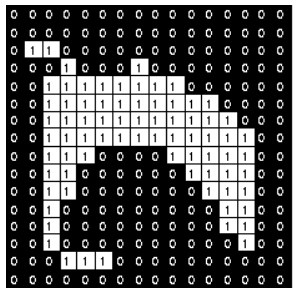
\includegraphics[width=0.5\textwidth]{region-example.png}
        \caption{In white a region.}
      \end{figure}
    \end{column}
    \begin{column}{0.5\textwidth}
      \begin{figure}
        \centering
        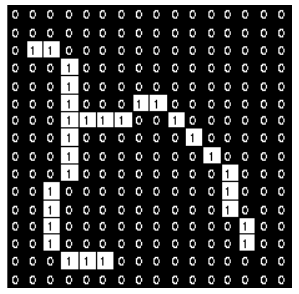
\includegraphics[width=0.5\textwidth]{skel-region-example.png}
        \caption{The skeleton of the region on the left.}
      \end{figure}
    \end{column}
  \end{columns}
\end{frame}

\begin{frame}
  \frametitle{Zhang-Suen Parallalel Thinning}
  \begin{itemize}
    \item Given an element $P_1 = M[i][j]$, its neighbours are:
          \begin{center}
            \setlength{\arrayrulewidth}{0.3mm}
            \renewcommand{\arraystretch}{2}
            \begin{tabular}{|c|c|c|}
              \hline
              $P_9 = M[i-1][j-1]$ & $P_2 = M[i-1][j]$ & $P_3 = M[i-1][j+1]$ \\
              \hline
              $P_8 = M[i][j-1]$   & $P_1 = M[i][j]$   & $P_4 = M[i][j+1]$   \\
              \hline
              $P_7 = M[i+1][j-1]$ & $P_6 = M[i+1][j]$ & $P_5 = M[i+1][j+1]$ \\
              \hline
            \end{tabular}
          \end{center}

          \vspace{0.5cm}
    \item The algorithm iteratively removes all countour points (change the value from 1 to 0) which satisfy some conditions on their 8 neighbours.
          \\~\\
    \item The new value of a pixel at the $n$-th iteration is based on the values of its neighbours at the $n-1$-th iteration. This allows all pixel to be processed in \textbf{parallel} in each iteration.
  \end{itemize}
\end{frame}

\begin{frame}
  \frametitle{Pixel Deletion Conditions}
  \begin{itemize}
    \item An iteration (full pass over all the pixels) is divided in two sub-iterations.
          \\~\\
    \item \textbf{Sub-iteration 1}: $P_1$ is deleted if
          \begin{enumerate}
            \item $2 \leq B(P_1) \leq 6$
            \item $A(P_1) = 1$
            \item $P_2 * P_4 * P_6 = 0$
            \item $P_4 * P_6 * P_8 = 0$
          \end{enumerate}
          \vspace{0.3cm}
    \item \textbf{Sub-iteration 2}: $P_1$ is deleted if
          \begin{enumerate}
            \item Conditions 1 and 2 are true
            \item $P_2 * P_4 * P_8 = 0$
            \item $P_2 * P_6 * P_8 = 0$
          \end{enumerate}
          \vspace{0.3cm}
    \item $B(P_1)$ is the number of \textbf{1-value neighbours} of $P_1$. Condition 1 is needed to \textbf{preserve an endpoint} of the skeleton.
    \item $A(P_1)$ is the number of \textbf{0-1 patterns} in the ordered sequence of neighbours $P_2, P_3, \dots, P_9, P_2$. Condition 2 is needed to preserve \textbf{connectivity}, i.e. not split the skeleton in two.
  \end{itemize}
\end{frame}

\begin{frame}
  \frametitle{Pixel Deletion Conditions}
  \begin{figure}
    \centering
    \begin{subfigure}[b]{0.3\textwidth}
      \centering
      
\includegraphics[width=\textwidth]{simple-zhang/img_000.png}
      \caption{Original image.}
    \end{subfigure}
    \hfill
    \begin{subfigure}[b]{0.3\textwidth}
      \centering
      
\includegraphics[width=\textwidth]{simple-zhang/img_011.png}
      \caption{After sub-iteration 1.}
    \end{subfigure}
    \hfill
    \begin{subfigure}[b]{0.3\textwidth}
      \centering
      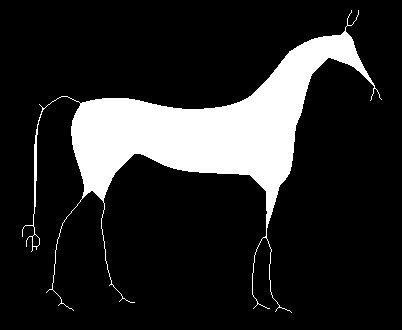
\includegraphics[width=\textwidth]{simple-zhang/img_014.png}
      \caption{After sub-iteration 2.}
    \end{subfigure}
    \caption{Effects of one single iteration on an example image.}
  \end{figure}
  Thanks to conditions 3 and 4:
  \begin{itemize}
    \item Sub-iteration 1 removes East and South boundary pixels and North-West corner pixels.
    \item Sub-iteration 2 removes West and North boundary pixels and South-East corner pixels.
  \end{itemize}
\end{frame}

\begin{frame}[c]
  \frametitle{Zhang-Suen Visualization}
  \centering
  \begin{figure}
  \animategraphics[loop, autoplay,width=0.5\textwidth]{15}{../stepbystep_exec/zhang/img_}{000}{047}
  \caption{Animation of Zhang-Suen algorithm removing contour pixels until only the skeleton remains.}
  \end{figure}
\end{frame}

\begin{frame}
  \frametitle{Zhang-Suen Pseudocode}
  \section{Zhang-Suen Parallalel Thinning}
\begin{frame}
  \frametitle{Zhang-Suen Parallalel Thinning}
  \textbf{Zhang-Suen algorithm}~\cite{zha84} is a fast parallel algorithm which takes a binary 2D image and removes pixels from the object's border by making successive iterations until convergence.
  \begin{block}{2D Binary image}
    A matrix $M$ where each pixel $M[i][j]$ is either $1$ or $0$. A \textbf{region} in an image is a connected set of $1$-valued pixels.
  \end{block}
  \begin{columns}
    \begin{column}{0.5\textwidth}
      \begin{figure}
        \centering
        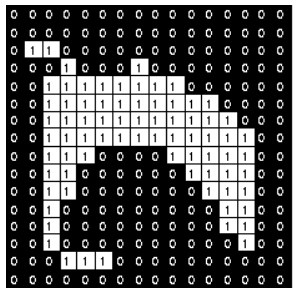
\includegraphics[width=0.5\textwidth]{region-example.png}
        \caption{In white a region.}
      \end{figure}
    \end{column}
    \begin{column}{0.5\textwidth}
      \begin{figure}
        \centering
        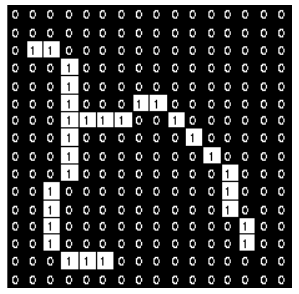
\includegraphics[width=0.5\textwidth]{skel-region-example.png}
        \caption{The skeleton of the region on the left.}
      \end{figure}
    \end{column}
  \end{columns}
\end{frame}

\begin{frame}
  \frametitle{Zhang-Suen Parallalel Thinning}
  \begin{itemize}
    \item Given an element $P_1 = M[i][j]$, its neighbours are:
          \begin{center}
            \setlength{\arrayrulewidth}{0.3mm}
            \renewcommand{\arraystretch}{2}
            \begin{tabular}{|c|c|c|}
              \hline
              $P_9 = M[i-1][j-1]$ & $P_2 = M[i-1][j]$ & $P_3 = M[i-1][j+1]$ \\
              \hline
              $P_8 = M[i][j-1]$   & $P_1 = M[i][j]$   & $P_4 = M[i][j+1]$   \\
              \hline
              $P_7 = M[i+1][j-1]$ & $P_6 = M[i+1][j]$ & $P_5 = M[i+1][j+1]$ \\
              \hline
            \end{tabular}
          \end{center}

          \vspace{0.5cm}
    \item The algorithm iteratively removes all countour points (change the value from 1 to 0) which satisfy some conditions on their 8 neighbours.
          \\~\\
    \item The new value of a pixel at the $n$-th iteration is based on the values of its neighbours at the $n-1$-th iteration. This allows all pixel to be processed in \textbf{parallel} in each iteration.
  \end{itemize}
\end{frame}

\begin{frame}
  \frametitle{Pixel Deletion Conditions}
  \begin{itemize}
    \item An iteration (full pass over all the pixels) is divided in two sub-iterations.
          \\~\\
    \item \textbf{Sub-iteration 1}: $P_1$ is deleted if
          \begin{enumerate}
            \item $2 \leq B(P_1) \leq 6$
            \item $A(P_1) = 1$
            \item $P_2 * P_4 * P_6 = 0$
            \item $P_4 * P_6 * P_8 = 0$
          \end{enumerate}
          \vspace{0.3cm}
    \item \textbf{Sub-iteration 2}: $P_1$ is deleted if
          \begin{enumerate}
            \item Conditions 1 and 2 are true
            \item $P_2 * P_4 * P_8 = 0$
            \item $P_2 * P_6 * P_8 = 0$
          \end{enumerate}
          \vspace{0.3cm}
    \item $B(P_1)$ is the number of \textbf{1-value neighbours} of $P_1$. Condition 1 is needed to textbf{preserve an endpoint} of the skeleton.
    \item $A(P_1)$ is the number of \textbf{0-1 patterns} in the ordered sequence of neighbours $P_2, P_3, \dots, P_9, P_2$. Condition 2 is needed to preserve \textbf{connectivity}, i.e. not split the skeleton in two.
  \end{itemize}
\end{frame}

\begin{frame}
  \frametitle{Pixel Deletion Conditions}
  \begin{figure}
    \centering
    \begin{subfigure}[b]{0.3\textwidth}
      \centering
      
\includegraphics[width=\textwidth]{simple-zhang/img_000.png}
      \caption{Original image.}
    \end{subfigure}
    \hfill
    \begin{subfigure}[b]{0.3\textwidth}
      \centering
      
\includegraphics[width=\textwidth]{simple-zhang/img_011.png}
      \caption{After sub-iteration 1.}
    \end{subfigure}
    \hfill
    \begin{subfigure}[b]{0.3\textwidth}
      \centering
      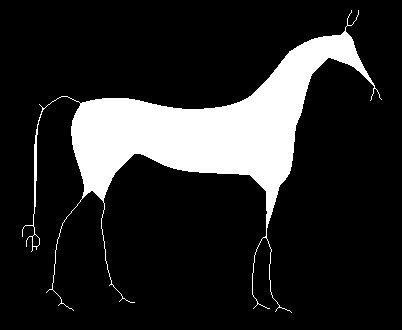
\includegraphics[width=\textwidth]{simple-zhang/img_014.png}
      \caption{After sub-iteration 2.}
    \end{subfigure}
    \caption{Effects of one single iteration on an example image.}
  \end{figure}
  Thanks to conditions 3 and 4:
  \begin{itemize}
    \item Sub-iteration 1 removes East and South boundary pixels and North-West corner pixels.
    \item Sub-iteration 2 removes West and North boundary pixels and South-East corner pixels.
  \end{itemize}
\end{frame}

\begin{frame}[c]
  \frametitle{Zhang-Suen Visualization}
  \centering
  \begin{figure}
  \animategraphics[loop, autoplay,width=0.5\textwidth]{15}{../zhang/img_}{000}{047}
  \caption{Animation of Zhang-Suen algorithm removing contour pixels until only the skeleton remains.}
  \end{figure}
\end{frame}

\begin{frame}
  \frametitle{Zhang-Suen Pseudocode}
  \section{Zhang-Suen Parallalel Thinning}
\begin{frame}
  \frametitle{Zhang-Suen Parallalel Thinning}
  \textbf{Zhang-Suen algorithm}~\cite{zha84} is a fast parallel algorithm which takes a binary 2D image and removes pixels from the object's border by making successive iterations until convergence.
  \begin{block}{2D Binary image}
    A matrix $M$ where each pixel $M[i][j]$ is either $1$ or $0$. A \textbf{region} in an image is a connected set of $1$-valued pixels.
  \end{block}
  \begin{columns}
    \begin{column}{0.5\textwidth}
      \begin{figure}
        \centering
        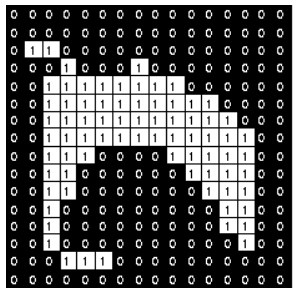
\includegraphics[width=0.5\textwidth]{region-example.png}
        \caption{In white a region.}
      \end{figure}
    \end{column}
    \begin{column}{0.5\textwidth}
      \begin{figure}
        \centering
        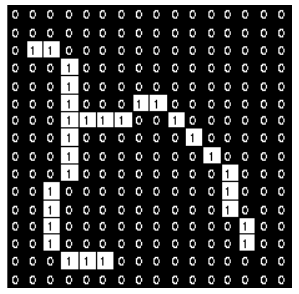
\includegraphics[width=0.5\textwidth]{skel-region-example.png}
        \caption{The skeleton of the region on the left.}
      \end{figure}
    \end{column}
  \end{columns}
\end{frame}

\begin{frame}
  \frametitle{Zhang-Suen Parallalel Thinning}
  \begin{itemize}
    \item Given an element $P_1 = M[i][j]$, its neighbours are:
          \begin{center}
            \setlength{\arrayrulewidth}{0.3mm}
            \renewcommand{\arraystretch}{2}
            \begin{tabular}{|c|c|c|}
              \hline
              $P_9 = M[i-1][j-1]$ & $P_2 = M[i-1][j]$ & $P_3 = M[i-1][j+1]$ \\
              \hline
              $P_8 = M[i][j-1]$   & $P_1 = M[i][j]$   & $P_4 = M[i][j+1]$   \\
              \hline
              $P_7 = M[i+1][j-1]$ & $P_6 = M[i+1][j]$ & $P_5 = M[i+1][j+1]$ \\
              \hline
            \end{tabular}
          \end{center}

          \vspace{0.5cm}
    \item The algorithm iteratively removes all countour points (change the value from 1 to 0) which satisfy some conditions on their 8 neighbours.
          \\~\\
    \item The new value of a pixel at the $n$-th iteration is based on the values of its neighbours at the $n-1$-th iteration. This allows all pixel to be processed in \textbf{parallel} in each iteration.
  \end{itemize}
\end{frame}

\begin{frame}
  \frametitle{Pixel Deletion Conditions}
  \begin{itemize}
    \item An iteration (full pass over all the pixels) is divided in two sub-iterations.
          \\~\\
    \item \textbf{Sub-iteration 1}: $P_1$ is deleted if
          \begin{enumerate}
            \item $2 \leq B(P_1) \leq 6$
            \item $A(P_1) = 1$
            \item $P_2 * P_4 * P_6 = 0$
            \item $P_4 * P_6 * P_8 = 0$
          \end{enumerate}
          \vspace{0.3cm}
    \item \textbf{Sub-iteration 2}: $P_1$ is deleted if
          \begin{enumerate}
            \item Conditions 1 and 2 are true
            \item $P_2 * P_4 * P_8 = 0$
            \item $P_2 * P_6 * P_8 = 0$
          \end{enumerate}
          \vspace{0.3cm}
    \item $B(P_1)$ is the number of \textbf{1-value neighbours} of $P_1$. Condition 1 is needed to textbf{preserve an endpoint} of the skeleton.
    \item $A(P_1)$ is the number of \textbf{0-1 patterns} in the ordered sequence of neighbours $P_2, P_3, \dots, P_9, P_2$. Condition 2 is needed to preserve \textbf{connectivity}, i.e. not split the skeleton in two.
  \end{itemize}
\end{frame}

\begin{frame}
  \frametitle{Pixel Deletion Conditions}
  \begin{figure}
    \centering
    \begin{subfigure}[b]{0.3\textwidth}
      \centering
      
\includegraphics[width=\textwidth]{simple-zhang/img_000.png}
      \caption{Original image.}
    \end{subfigure}
    \hfill
    \begin{subfigure}[b]{0.3\textwidth}
      \centering
      
\includegraphics[width=\textwidth]{simple-zhang/img_011.png}
      \caption{After sub-iteration 1.}
    \end{subfigure}
    \hfill
    \begin{subfigure}[b]{0.3\textwidth}
      \centering
      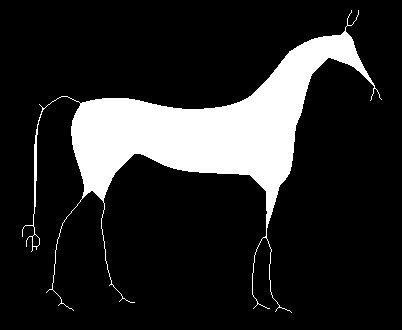
\includegraphics[width=\textwidth]{simple-zhang/img_014.png}
      \caption{After sub-iteration 2.}
    \end{subfigure}
    \caption{Effects of one single iteration on an example image.}
  \end{figure}
  Thanks to conditions 3 and 4:
  \begin{itemize}
    \item Sub-iteration 1 removes East and South boundary pixels and North-West corner pixels.
    \item Sub-iteration 2 removes West and North boundary pixels and South-East corner pixels.
  \end{itemize}
\end{frame}

\begin{frame}[c]
  \frametitle{Zhang-Suen Visualization}
  \centering
  \begin{figure}
  \animategraphics[loop, autoplay,width=0.5\textwidth]{15}{../zhang/img_}{000}{047}
  \caption{Animation of Zhang-Suen algorithm removing contour pixels until only the skeleton remains.}
  \end{figure}
\end{frame}

\begin{frame}
  \frametitle{Zhang-Suen Pseudocode}
  \section{Zhang-Suen Parallalel Thinning}
\begin{frame}
  \frametitle{Zhang-Suen Parallalel Thinning}
  \textbf{Zhang-Suen algorithm}~\cite{zha84} is a fast parallel algorithm which takes a binary 2D image and removes pixels from the object's border by making successive iterations until convergence.
  \begin{block}{2D Binary image}
    A matrix $M$ where each pixel $M[i][j]$ is either $1$ or $0$. A \textbf{region} in an image is a connected set of $1$-valued pixels.
  \end{block}
  \begin{columns}
    \begin{column}{0.5\textwidth}
      \begin{figure}
        \centering
        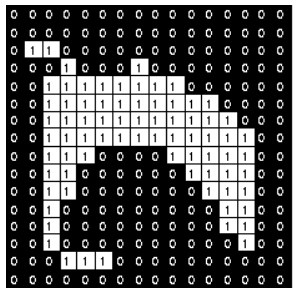
\includegraphics[width=0.5\textwidth]{region-example.png}
        \caption{In white a region.}
      \end{figure}
    \end{column}
    \begin{column}{0.5\textwidth}
      \begin{figure}
        \centering
        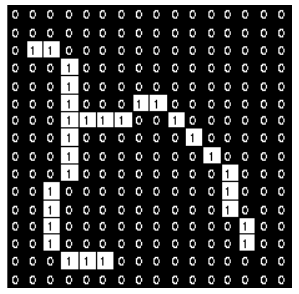
\includegraphics[width=0.5\textwidth]{skel-region-example.png}
        \caption{The skeleton of the region on the left.}
      \end{figure}
    \end{column}
  \end{columns}
\end{frame}

\begin{frame}
  \frametitle{Zhang-Suen Parallalel Thinning}
  \begin{itemize}
    \item Given an element $P_1 = M[i][j]$, its neighbours are:
          \begin{center}
            \setlength{\arrayrulewidth}{0.3mm}
            \renewcommand{\arraystretch}{2}
            \begin{tabular}{|c|c|c|}
              \hline
              $P_9 = M[i-1][j-1]$ & $P_2 = M[i-1][j]$ & $P_3 = M[i-1][j+1]$ \\
              \hline
              $P_8 = M[i][j-1]$   & $P_1 = M[i][j]$   & $P_4 = M[i][j+1]$   \\
              \hline
              $P_7 = M[i+1][j-1]$ & $P_6 = M[i+1][j]$ & $P_5 = M[i+1][j+1]$ \\
              \hline
            \end{tabular}
          \end{center}

          \vspace{0.5cm}
    \item The algorithm iteratively removes all countour points (change the value from 1 to 0) which satisfy some conditions on their 8 neighbours.
          \\~\\
    \item The new value of a pixel at the $n$-th iteration is based on the values of its neighbours at the $n-1$-th iteration. This allows all pixel to be processed in \textbf{parallel} in each iteration.
  \end{itemize}
\end{frame}

\begin{frame}
  \frametitle{Pixel Deletion Conditions}
  \begin{itemize}
    \item An iteration (full pass over all the pixels) is divided in two sub-iterations.
          \\~\\
    \item \textbf{Sub-iteration 1}: $P_1$ is deleted if
          \begin{enumerate}
            \item $2 \leq B(P_1) \leq 6$
            \item $A(P_1) = 1$
            \item $P_2 * P_4 * P_6 = 0$
            \item $P_4 * P_6 * P_8 = 0$
          \end{enumerate}
          \vspace{0.3cm}
    \item \textbf{Sub-iteration 2}: $P_1$ is deleted if
          \begin{enumerate}
            \item Conditions 1 and 2 are true
            \item $P_2 * P_4 * P_8 = 0$
            \item $P_2 * P_6 * P_8 = 0$
          \end{enumerate}
          \vspace{0.3cm}
    \item $B(P_1)$ is the number of \textbf{1-value neighbours} of $P_1$. Condition 1 is needed to textbf{preserve an endpoint} of the skeleton.
    \item $A(P_1)$ is the number of \textbf{0-1 patterns} in the ordered sequence of neighbours $P_2, P_3, \dots, P_9, P_2$. Condition 2 is needed to preserve \textbf{connectivity}, i.e. not split the skeleton in two.
  \end{itemize}
\end{frame}

\begin{frame}
  \frametitle{Pixel Deletion Conditions}
  \begin{figure}
    \centering
    \begin{subfigure}[b]{0.3\textwidth}
      \centering
      
\includegraphics[width=\textwidth]{simple-zhang/img_000.png}
      \caption{Original image.}
    \end{subfigure}
    \hfill
    \begin{subfigure}[b]{0.3\textwidth}
      \centering
      
\includegraphics[width=\textwidth]{simple-zhang/img_011.png}
      \caption{After sub-iteration 1.}
    \end{subfigure}
    \hfill
    \begin{subfigure}[b]{0.3\textwidth}
      \centering
      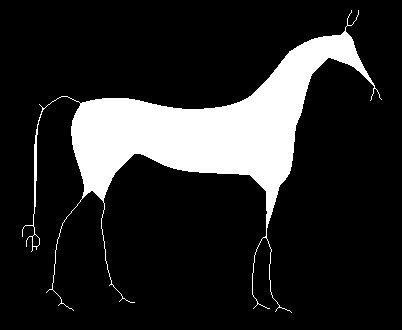
\includegraphics[width=\textwidth]{simple-zhang/img_014.png}
      \caption{After sub-iteration 2.}
    \end{subfigure}
    \caption{Effects of one single iteration on an example image.}
  \end{figure}
  Thanks to conditions 3 and 4:
  \begin{itemize}
    \item Sub-iteration 1 removes East and South boundary pixels and North-West corner pixels.
    \item Sub-iteration 2 removes West and North boundary pixels and South-East corner pixels.
  \end{itemize}
\end{frame}

\begin{frame}[c]
  \frametitle{Zhang-Suen Visualization}
  \centering
  \begin{figure}
  \animategraphics[loop, autoplay,width=0.5\textwidth]{15}{../zhang/img_}{000}{047}
  \caption{Animation of Zhang-Suen algorithm removing contour pixels until only the skeleton remains.}
  \end{figure}
\end{frame}

\begin{frame}
  \frametitle{Zhang-Suen Pseudocode}
  \input{assets/pseudocode/zhang.tex}
\end{frame}

\end{frame}

\end{frame}

\end{frame}
